\section{Закрытие программы}
\begin{enumerate}[\thesection .1]
	\item В главном меню <<Оптимы>> (рис.\ref{pic:picgl}) в правом верхнем углу можно заметить значок <<Замочек>>.(1) В нормальном состоянии он слегка приоткрыт. Это говорит о том, что с системой можно работать.(рис.\ref{pic:pic7_1})
    При закрытии программы стандартными средствами Android с помощью стрелки назад выводится следующее сообщение о том что при выходе из программы будет произведено закрытие дня. Если выбрать утвердительный ответ,то программа закроется и при следующем открытии <<Замочек>> будет закрыт и никакие действия в программе невозможны. Для решения этой проблемы необходимо звонить в отдел IT или своему непосредственному руководителю.
    \begin{figure}[H]
    	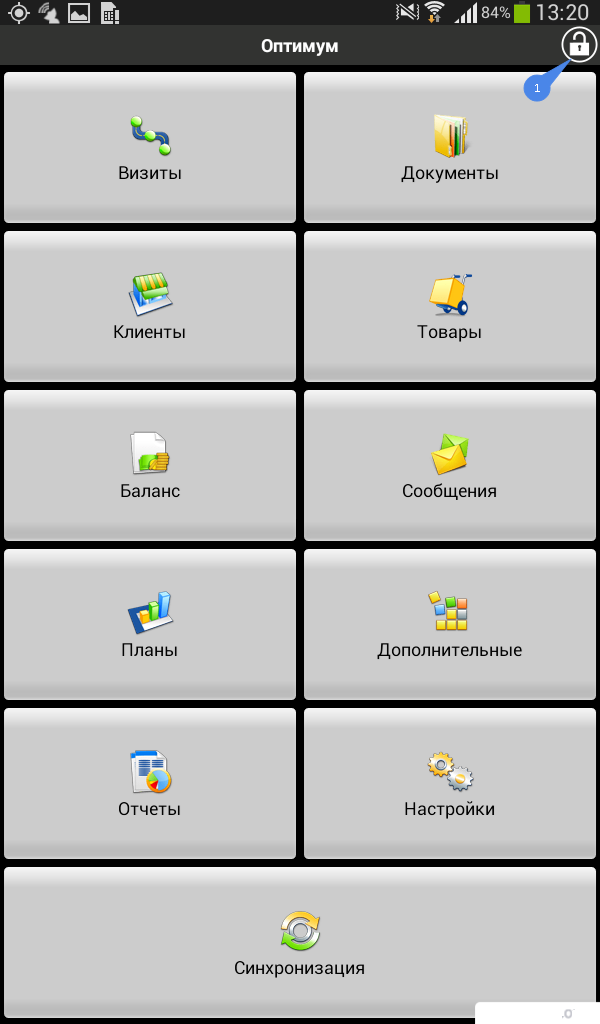
\includegraphics[width=0.3\linewidth]{scr7_1.png} 
    	\caption{Программа разблокирована}\label{pic:pic7_1}
    \end{figure}
    \item Закрытие программы необходимо производить сворачиванием нажав на <<Домик>>.	
\end{enumerate}